\documentclass[letterpaper,twoside,onecolumn,openright,final]{memoir}
%    vs.       others...   oneside twocolumn openleft  draft showtrims
%                          twoside onecolumn openany   ms
%                                            openright final 
\input lumos_common
\begin{document}
\frontmatter

\thispagestyle{empty}
\ThisLLCornerWallPaper{1}{images/cover}
%\strut
\vfill
\begin{center}
{\HUGE Installing the Lumos\TM}

\bigskip

{\HUGE 24-Channel DC Controller}

\vfill

\end{center}

\newpage
\begin{center}
\LLimg[width=1in]{danger-generic}

%DANGER! 

\mc{RISK OF FIRE, ELECTROCUTION, SERIOUS INJURY OR DEATH!} 
\end{center}

This circuit design, including but not limited to any associated plans, schematics, designs, board layouts, documentation, 
and/or components, is \mc{EXPERIMENTAL} and for \mc{EDUCATIONAL} purposes only. It is not a finished consumer-grade product.
It is assumed that you have the necessary understanding and skill to assemble and/or use electronic circuits.

Proceed \mc{ONLY} if you know exactly what you are doing, understand the proper procedures for working with the high voltage present on the components and PC boards, and understand that you do so \mc{ENTIRELY AT YOUR OWN RISK.}

The author makes \mc{NO} representation as to suitability or fitness for any purpose whatsoever, and disclaims any and all liability or warranty to the full extent permitted by applicable law.
\index{warranty, limitation of}
\index{danger warnings}
\index{warnings}

\strut\vfill
\noindent Edition 1.0, for Lumos 24-Channel DC Controller circuit version 1.0.8.

\smallskip


\noindent Copyright \copyright\ 2013 by Steven L. Willoughby,
Aloha, Oregon, USA.  All Rights Reserved.  
This document is released under the terms and conditions of the 
Creative Commons ``Attribution-NoDerivs 3.0 Unported'' license.  
In summary, you are free to use, reproduce, and redistribute this 
document provided you give full attribution to its author and do not
alter it or create derivative works from it.  See
\URL{http://creativecommons.org/licenses/by\-nd\-/\-3.0/} for the full
set of licensing terms.

\begin{center}
\LLimg[width=.5in]{cc}\LLimg[width=.5in]{by}\LLimg[width=.5in]{nd}
\end{center}

\newpage
\tableofcontents

\mainmatter

\chapter{Introduction}
\LLstart{C}{ongratulations}{on joining} the many computer-controlled
Christmas light enthusiasts, \ix{theatrical lighting} technicians, electronics hobbyists,
\index{Christmas lights}
and home automation innovators who are experimenting with new ways to have computers
control lights and other electronic devices.

The Lumos\TM\ 24-Channel DC Controller board places 24 such devices under the control
of your computer.  These outputs are arranged into three \ix{blocks} of eight \ix{channels}.
Each block is electrically isolated from the logic control circuit and from each other,
so each block may be separately powered at different voltages if desired.

If Lumos boards are configured with the \ix{RS-485} network option, up to sixteen Lumos
boards may be ``daisy chained'' together (a total of 384 channels) and controlled from 
the same PC serial port.
By plugging DC-powered Christmas lights into the Lumos controller, your PC can orchestrate
a dazzling display of lights synchronized to music.

This manual assumes you have a Lumos controller board built and ready to put into operation.
We will describe how to install it in a working circuit.  

The operational details involved
in getting the controller to work with software is described in 
\emph{Using Lumos\TM\ SSR Controllers.}

\section{Intended Audience}
This is an ``advanced'' level do-it-yourself electronic circuit project.  It is not
an off-the-shelf consumer-ready product.  It is only designed for educational and experimental
use by experienced hobbyists and professionals who possess the skill to construct electronic
\marginpar{\centerline{\LLimg[height=.5in]{danger-sign}}}
circuits, to understand how they function, troubleshoot problems with them, and to use them safely.

\section{Limitation of Warranty}
\index{danger warnings}
\index{warnings}
\index{warranty, limitation of}
Since this is a do-it-yourself project, the quality of the final product, and whether it 
functions as intended, is largely a result of your own efforts in building it.  As such, we
cannot offer to troubleshoot, repair, or replace a board we did not assemble for you.  Accordingly,
\marginpar{\centerline{\LLimg[height=.5in]{danger-sign}}}
these instructions, and all accompanying plans, schematics, software, hardware, and other
project materials are provided to you ``\mc{AS-IS}'' at no cost, as a courtesy between 
\acronym{DIY} hobbyists with \mc{NO WARRANTY} of any kind expressed or implied.  If you proceed
to build and/or use this unit, you do so \mc{ENTIRELY AT YOUR OWN RISK}.

If you purchased hardware materials from us (such as a PC board or programmed controller chip),
we will---at our sole discretion---replace, repair, or refund the cost of those materials if they were defective in manufacture
as shipped to you, up to 90~days from the date they were shipped to you, 
but are not liable for damage caused by your handling or assembly of the unit.
Otherwise, we make no representation of suitability or fitness for any particular purpose and disclaim
all other warranty or liability of any kind to the full extent permitted by law.

%\section{How to Use this Manual}
%Please begin by reviewing the safety information in Chapter~\ref{ch:safety}.  

%When you are ready to begin assembling your Lumos controller, gather the required tools and materials
%as explained in Chapter~\ref{ch:materials}.  
%
%Then read carefully the \emph{entire} set of instructions in Chapter~\ref{ch:assembly} \emph{before}
%beginning any actual work.  Begin assembly \emph{only} if you understand all the steps you will need
%to carry out.


\section{The Name of the Game}
The name ``Lumos'' is a combination of \emph{lumen}, the Latin word for ``light,''
and the initial letters of ``Orchestration System.''  Hence, ``Light Orchestration System''
which is the most common application for which the Lumos hardware and software are used---running
computerized lighting displays.



\chapter{Safety Information}\label{ch:safety}

\LLstart{B}{efore}{you begin installing} your Lumos controller, please take the time to
carefully read the following \ix{safety precautions}.  Failure to follow this advice could
result in death or serious injury, damage to the Lumos controller unit, and/or damage
to the other devices plugged into the controller.
\index{danger warnings}
\index{warnings}

%\section{Hazardous Materials}
%While assembling this unit you may come in contact with \ix{hazardous chemicals}.  The Lumos
%product contains no hazardous parts \emph{per se} but if you choose to assemble it using
%lead-based solder, you may expose yourself to risk of \ix{lead poisoning}.  The main cause of lead
%poisoning due to soldering is by ingesting lead particles left on your hands or work surface.
%To avoid this, keep food away from your work area, and thoroughly wash your hands and work
%surfaces before handling food.
%\marginpar{\LLimg[width=1in]{poison_sign}}
%
%In addition, if you choose to use other chemical agents (e.g., to clean excess flux from your
%soldered board), be sure to read and follow their precautions and instructions carefully.

\section{Small Part Danger}
This board contains small parts which could pose a \ix{choking hazard} to small children.
This product is not a toy and is not intended for use by children in any circumstance.
The small parts on the product can be swallowed by children under 4~years of age. Keep
\marginpar{\centerline{\LLimg[height=.5in]{danger-generic}}}
out of reach of children.

\section{Hazardous Voltage}
Exercise care when working with any electrical system, including one such as the Lumos DC
controllers (even though in theory they deal with low voltages).  The power supplies of the
loads plugged into the Lumos controller, and even the power loads being controlled, may present
\marginpar{\centerline{\LLimg[width=.5in]{danger-shock}}}
a \ix{shock hazard} if not wired and handled using standard safety protocols.  Never touch or work
with live circuits. Always disconnect the power source before working on your Lumos controller.

When working with loads outdoors, be sure all supplies are plugged into \acronym{GFIC}-protected
circuits.

%\section{Physical Hazards}
%While assembling the unit, always wear \acronym{ANSI}-approved \ix{eye protection} gear.  When soldering,
%always be aware of---and in control of---the location of your soldering iron (it will be 300$^\circ$F--500$^\circ$F---any slight 
%mistake can be costly, painful, or dangerous)! Bits of molten metal or flux can spatter onto your
%skin or in your eyes during soldering.  When cutting leads, sharp metal wires may be launched into the
%air, and could hit your eyes.
%\marginpar{\LLimg[width=1in]{danger-sign}}

\section{Electrostatic Discharge (ESD) Warning}
Many of the components used in this project are sensitive to static electricity.  Always use a proper
\acronym{ESD}-safe work environment when handling them, or these parts may be permanently damaged.  If
a part is damaged in this way, 
\marginpar{\centerline{\LLimg[height=.5in]{esd_symbol_l}}}
it is impossible to tell by looking at the part, and you won't necessarily
feel the \ix{static discharge} which caused the damage.  Never take the risk of handling sensitive components
without \acronym{ESD} protection in place.
\index{danger warnings}
\index{warnings}

These parts include all transistors (Q0--Q23), voltage regulators (U6--U8 and U11), diodes (D0--D11),
and integrated circuits (U0--U5, U9--U10, and U12--U13).

\section{Circuit Loading}
Always respect the maximum voltage and current capacity of the board and your wiring.  Overloading any
\index{overloaded circuits}
\index{maximum limits}
of these may result serious injury, death, fire, and/or severe damage to any or all of the devices in use.

Each block of eight controlled loads may not exceed 
\marginpar{\centerline{\LLimg[height=.5in]{danger-sign}}}
10\,A total for the block.  
Each single output channel
may not exceed 5\,A.  These should be considered \emph{absolute maximum} tolerances.  The board was designed
to operate at sustained levels below those limits.

Also note that the Lumos output circuits were designed to control simple resistive loads such as
incandescent lights.  They are not appropriate for all kinds of loads.  Some inductive loads
(for example, electromagnetic relays and motors) may require a protective ``snubber'' circuit
between the Lumos output and the load to avoid damage to the Lumos board and/or the attached load.

%\chapter{What You Will Need}\label{ch:materials}
%
%\LLstart{A}{SSEMBLING}{this project} requires soldering approximately 140 components onto a PC board.\footnote{The actual number will vary depending on the options selected.}  Before beginning construction, be sure you have the following tools and materials on hand:
%\begin{itemize}
%	\item A Lumos 24-Channel DC Controller \ix{PC board}. 
%		These instructions are intended for version
%		1.0 of this board, which includes boards numbrered ``1.0.$x$'' where $x$ is any
%		number.  If your board has a different version number printed on it, you need an
%		instruction manual which was written for that board type.  \mc{DO NOT} proceed to
%		use these instructions for that board!
%		\index{PC board!versions}
%	\item All the electronic \ix{components} required for the board.  These are listed in the
%		following table.
%	\item A \ix{soldering iron} with thin ``pencil'' tip.
%	\item Rosin-core \ix{solder}.  
%	\item Diagonal \ix{wire cutters}.
%	\item \mc{ESD} protection gear such as an anti-static \ix{grounding strap}.
%	\item IC \ix{chip insertion tools}.
%	\item Needle-nose \ix{pliers}.
%	\item A few ounces of thermal (heat sink) grease.
%\end{itemize}
%
%\begin{longtable}[c]{|r|l|l|}\hline
%\multicolumn{3}{|c|}{\bfseries Bill of Materials}\\\hline
%{\bfseries Qty} & {\bfseries Number} & {\bfseries Description} \\\hline\hline
%3 & C0--C2 & Capacitors, 0.33$\mu$F \\
%3 & C3--C5 & Capacitors, 0.1$\mu$F \\\hline
%3 & D0--D2 & Diodes, 1N4004 \\
%3 & D3--D5 & \mc{LED}, green, 3\,mm \\\hline
%3 & F0--F2 & Fuse, 10\,A, with holder \\\hline
%2 & HS0, HS1& Heat sinks, aluminum \\\hline
%3 & J0--J2 & Terminal block, 10-position \\
%3 & J3--J5 & Terminal block, 2-position \\
%3 & J6--J8 & Jumper block header, 4-position \\\hline
%24& Q0--Q23& Transistor, \acronym{MOSFET} \\\hline
%6 & R0--R5 & Resistor network, 680$\Omega\times$5 \\
%3 & R6--R8 & Resistor, 200$\Omega$, \sfrac{1}{4}\,W \\
%24& R9--R32& Resistor, 470$\Omega$, \sfrac{1}{4}\,W \\
%24&R33--R56& Resistor, 10K, \sfrac{1}{4}\,W\\\hline
%6 & U0--U5 & K847PH quad opto-isolator, \mc{NPN} transistor output \\
%3 & U6--U8 & LM78L05 +5\,V DC regulator \\
%6 & XU0--XU5 & \mc{DIP} socket, 16-pin \\\hline\hline
%24& XX0--XX23& \#4 bolts, \sfrac{3}{8}$''$ long, with lock washers and nuts\\\hline\hline
%\multicolumn{3}{|l|}{\emph{Built-in CPU Option}}\\\hline\hline
%2 & C6--C7 & Capacitors, 33pF \\
%2 & C8, C12& Capacitor, 0.1$\mu$F \\
%1 & C9     & Capacitor, 0.01$\mu$F \\
%1 & C11	   & Capacitor, 0.33$\mu$F \\\hline
%1 & D6     & Diode, 1N4004 \\
%2 & D7, D8 & \mc{LED}, green, 3\,mm \\
%2 & D9, D11& \mc{LED}, yellow, 3\,mm \\
%1 & D10    & \mc{LED}, red, 3\,mm \\\hline
%2 & J9, J10& Terminal block, 2-position \\
%1 & J11	   & Jumper block header, 5-position \\
%1 & J17    & Jumper block header, 4-position \\\hline
%1 & R57    & Resistor, 33K, \sfrac{1}{4}\,W \\
%1 & R58    & Resistor, 10K, \sfrac{1}{4}\,W \\
%1 & R60    & Resistor network, 220$\Omega\times$5, \sfrac{1}{4}\,W \\
%1 & R61    & Resistor, 330$\Omega$, \sfrac{1}{4}\,W \\\hline
%1 & S0     & Push-button, red, ``reset'' \\
%1 & S1     & Push-button, green, ``option'' \\\hline
%1 & U9     & PIC18F4685 microcontroller, Lumos programmed \\
%1 & U11    & LM7805 +5\,V DC regulator \\\hline
%1 & X0     & Crystal, 10\,MHz \\\hline
%1 & XU9    & \mc{DIP} socket, 40-pin \\\hline\hline
%\multicolumn{3}{|l|}{\emph{RS-485 Communications Options}}\\\hline\hline
%1 & C10    & Capacitor, 0.01$\mu$F \\\hline
%1 & F3	   & Fuse, 800\,mA, with holder \\\hline
%2 & J12, J13& Modular jack, 8p8c \\\hline
%1 & R62    & Resistor, 10K, \sfrac{1}{4}\,W \\
%1 & R63    & Resistor, 100$\Omega$, \sfrac{1}{4}\,W \\\hline
%1 & U10    & SN75176 RS-485 driver/receiver; \emph{half-duplex option only} \\
%1 & U13    & MAX489 RS-485 driver/receiver; \emph{full-duplex option only} \\\hline
%1 & XU10   & \mc{DIP} socket, 8-pin; \emph{half-duplex option only} \\
%1 & XU13   & \mc{DIP} socket, 14-pin; \emph{full-duplex option only} \\\hline\hline
%\multicolumn{3}{|l|}{\emph{RS-232 Communications Option}}\\\hline\hline
%1 & C13    & Capacitor, 1$\mu$F, electrolytic \\\hline
%1 & J15	   & Connector, D-sub-miniature DE-9, female \\\hline
%1 & U12    & MAX233A RS-232 driver/receiver\\\hline
%1 & XU12   & \mc{DIP} socket, 20-pin\\\hline\hline
%\multicolumn{3}{|l|}{\emph{Relay-Only Option}}\\\hline\hline
%1 & J14    & Ribbon cable box header, 26-position \\\hline\hline
%\multicolumn{3}{|l|}{\emph{Sensor Input Option}}\\\hline\hline
%1 & J16	   & Terminal block, 5-position; \emph{replaces J9}\\\hline
%1 & R59    & Resistor network, 10K$\times$5; \emph{replaces R58}\\\hline\hline
%\multicolumn{3}{|l|}{\emph{Logic-Level Output Option}}\\\hline\hline
%1 & J18    & Terminal block, 5-position\\\hline
%\end{longtable}
%
%\chapter{Assembling the PC Board}\label{ch:assembly}
%\LLstart{W}{ITH}{all the parts} and tools at hand as described in the previous chapter, you
%are now ready to begin assembly of the Lumos controller PC board.  The order of installation
%presented here is intended to make assembly as convenient as possible.  Generally this means
%progressing from the shortest to the tallest components, allowing the board to be laid flat
%face-down on the work surface while soldering the component leads.
%
%{\bfseries Note:} Take care to make good, solid \ix{solder connections} when installing components.
%Hold your soldering iron to the part's lead \emph{and} the \ix{annular ring} of the \acronym{PCB}
%until both are hot, then apply just enough solder to cover the ring, withdraw the solder, then 
%remove the heat.  Good solder connections should be shiny and smooth.
%
%{\bfseries Note:} The board layout is quite compact, with many components in a small space.  Take
%care when soldering that you don't accidentally heat the wrong component or form solder bridges between
%nearby contact points.
%
%\section{Determining Assembly Options}
%There are a number of different ways a Lumos 24-channel DC board may be constructed.  All boards
%will contain 24 output relays, so our assembly instructions will begin with the step-by-step 
%instructions for building this portion of the board (the entire lower half of the \acronym{PCB}).
%
%Following that, the instructions for completing the remainder of the board depend on the specific
%features you need.  These include:
%\begin{itemize}
%	\item	Simple ``relay mode'' with no intelligence built-in.  The relays will need to be
%		driven by an external controller capable of supplying 24 \acronym{TTL}-level
%		outputs (active low) as well as supplying +5\,V DC power to the Lumos board.
%	\item	Self-contained controller mode with built-in \acronym{CPU}.  It takes commands
%		from a host PC and manages the relay outputs directly.  This is the usual base 
%		configuration.  This requires one of the following communications options:
%		\begin{itemize}
%			\item	\ix{RS-232} communications---directly connected to the host PC's serial
%				port.  Allows 1 Lumos board at a distance of up to 25 feet.
%			\item	\ix{RS-485} communications---PC and Lumos boards on a serial network
%				of up to 16 Lumos boards at a distance of up to 1,200 meters
%				(4,000 feet).  This option is available in either full- or half-duplex
%				options.
%		\end{itemize}
%	\item	Sensor inputs \index{sensors} may be added to a Lumos board (except relay mode) to allow for external
%		sensors to trigger pre-programmed relay actions.  The host PC may also monitor the
%		sensors.
%	\item	Logic outputs \index{logic-level outputs} may be added to a Lumos board (except relay mode) to allow up to four
%		relay outputs as a \acronym{TTL}-level output to other controllers (such as a second
%		Lumos board's sensor inputs).
%\end{itemize}
%The specific instructions for adding those options to your Lumos board appear at the end of this 
%chapter.
%
%\section{Building the Relay Section}
%Refer to Figure~\ref{fig:placement} throughout these instructions to see where the components are 
%located on the \acronym{PCB}.  The locations are also labeled on the \acronym{PCB} itself.
%
%\begin{figure}
%\centerline{\LLimg{24dc-parts-placement}}
%\caption{Lumos Board Parts Placement Diagram\label{fig:placement}}
%\end{figure}
%
%\begin{enumerate}
%
%\item\label{s:resistor1}
%	Install (3) 220$\Omega$ \ix{resistors} in positions R6--R8 as marked on the \acronym{PCB}
%	and Figure~\ref{fig:placement}.  These have the color bands ``red-red-brown'' 
%	marking them.  Push them all the way until flush with the \acronym{PCB}.
%\item	solder their leads on the bottom side of the board.  
%\item\label{s:resistor2}
%	Trim the excess leads with \ix{diagonal cutters}.
%\item	Repeat steps \ref{s:resistor1}--\ref{s:resistor2} to 
%	install (24) 470$\Omega$ \ix{resistors} (``yellow-violet-brown'') at R9--R32.
%\item	Repeat steps \ref{s:resistor1}--\ref{s:resistor2}
%	to install (24) 10K \ix{resistors} (``brown-black-orange'') at R33--R56.
%\item	In the same fashion, install and solder (3) 0.33$\mu$F \ix{capacitors} into positions marked C0--C2.
%\item	Install and solder (3) 0.1$\mu$F capacitors into positions C3--C5.
%	{\bfseries NOTE: Capacitor C3 is located nearest to C0 on the \acronym{PCB}. On
%	board versions through 1.0.8, this is mis-labeled as ``C1.''}
%\item	Install (3) 1N4004 \ix{diodes} at D0--D2.  {\bfseries Note: These parts will not function
%	if inserted the wrong direction.} Each diode has
%	a stripe on one end. This end is inserted into the hole marked by the straight line (cathode)
%	drawn on the \acronym{PCB}.  The unmarked end goes into the hole marked by the triangle
%	(anode).  Solder into place. 
%\item	Install (3) green \acronym{LED}s at D3--D5.  {\bfseries Note: These must be inserted in the 
%	correct orientation.} The longer lead (anode) goes into the square hole, while the shorter
%	lead (cathode) goes into the round hole.  Solder into place.
%\item	Note the location of U0--U5 and R0--R5 (located \emph{inside} the borders of chips U0--U5).
%\item	Flip the board over to the bottom (solder) side.  Be sure you still see where R0--R5 are
%	located.
%\item\label{s:R0s}
%	Install (1) 680$\Omega$ \ix{resistor network} \emph{on the bottom (solder) side} of the board at
%	R0 (the row of six holes \emph{inside} U0).  {\bfseries Note the correct position of R0.} The
%	square hole on the \acronym{PCB} marks where pin~1 of R0 should be inserted.  Pin~1 is marked
%	with a dot on R0 itself
%	\marginpar{\LLimg[width=1in]{resistor-network}}
%\item	Holding R0 in place, carefully flip the board over.
%\item\label{s:R0e}
%	Keeping R0 straight, solder into place (soldering on the component side of the \acronym{PCB}).
%\item\label{s:R1}
%	Repeat steps \ref{s:R0s}--\ref{s:R0e} to install R1 on the bottom side of the \acronym{PCB},
%	inside U1's space.  {\bfseries Caution:} Pin~1 of R1 still goes in the square hole, but 
%	beware---this location is the mirror image of where it was for R0.  In other words, pin~1
%	of R0 and R1 are next to one another.
%\item	Repeat steps \ref{s:R0s}--\ref{s:R1} to install (4) more resistor networks at R2--R5.
%\item	Flip the board back over to the component side.  {\bfseries Caution:} From this point 
%	forward, don't forget those resistors are on the other side of the board.  If you press down
%	on the board (e.g., when installing chips into sockets), you will bend the resistors and may
%	break them.
%\item	Install (6) 16-pin \acronym{DIP} sockets XU0--XU5 in positions marked U0--U5.  
%	Note that they need to fit easily
%	over the soldered leads from R0--R5.  If they don't, select a different style of socket or
%	carefully trim down the resistor leads.
%\item	Solder sockets XU0--XU5.
%\item	Install (3) 4-position \ix{jumper block} headers at J6--J8.  Solder.
%\item	Install (3) LM78L05 voltage regulators at U6--U8.  Apply \ix{heat protection} while soldering in
%	place, and/or limit soldering time to 4 seconds or less.  Use \acronym{ESD} protection.
%\item	Install (3) \ix{fuse holders} at F0--F2.  Due to the wide \acronym{PCB} traces here, this may require
%	extra soldering time, but be careful not to overheat the parts.  The same will be true for
%	steps \ref{s:tb1}--\ref{s:tb2}.
%\item\label{s:tb1}
%	Install (3) 10-position terminal blocks at J0--J2.  
%\item\label{s:tb2}
%	Install (3) 2-position terminal blocks at J3--J5.
%\item\label{s:MOSFET1}
%	Using \acronym{ESD} protection, lay out (12) \acronym{MOSFET}s on your workbench.
%\item	Prepare each \acronym{MOSFET} by bending the middle lead 90$^\circ$ up then 90$^\circ$
%	back, so the lead has about 0.1$''$ offset between the middle pin and the others.  See
%	the illustration for details.  With the leads bent this way, the transistor should fit
%	easily into the holes at Q0 on the \acronym{PCB}.  See Figure~\ref{fig:mosfet}.
%\begin{figure}
%	\centerline{\LLimg[width=2in]{mosfet-side} \LLimg[width=2in]{mosfet-board}}
%	\caption{Bending the Pins of the M\mc{OSFET}s\label{fig:mosfet}}
%\end{figure}
%\item	Apply a \emph{small} dab of \ix{heat sink} grease on the back side of the transistor.
%\item\label{s:MOSFET2}
%	Bolt the transistor onto heat sink HS0, with the washer and nut on the transistor side,
%	making sure to smear the heat sink grease in a thin layer between the heat sink and
%	the transistor.  Make the part snug but not over-tight, and approximately 90$^\circ$
%	perpendicular to the heat sink bar.
%\item	Repeat steps \ref{s:MOSFET1}--\ref{s:MOSFET2} for the remaining transistors until you have
%	a row of 12 bolted to the heat sink.
%\item	Position the heat sink over all the even-numbered positions Q0--Q22 on the \acronym{PCB},
%	carefully adjusting the position of each part until all 36 pins slide into their holes.
%	Push the entire set very carefully into place until all transistors are seated as far as they
%	will go.  {\bfseries Note:} Due to irregularities in hole placement on the heat sink, it's
%	possible the transistors won't all be \emph{perfectly} straight, but they should be very
%	close to even and straight.
%\item	Using appropriate heat protection and/or limiting soldering time to 4 seconds or less per
%	pin, solder the leads of the 12 transistors into place.  
%\item\label{s:MOSFET3}
%	Trim the excess leads.
%\item	Repeat steps \ref{s:MOSFET1}--\ref{s:MOSFET3} for another 12 transistors, except:
%%with the following
%	changes:
%	\begin{itemize}
%		\item	Bolt them to the heat sink HS1 with the nut and washer on the side opposite the
%			transistor.
%		\item	Insert them into the odd-numbered locations Q1--Q23.
%		\item	When finished, there should be a slight air gap between the two rows of
%			transistors.
%	\end{itemize}
%\item	Insert (6) K847PH \ix{opto-isolator chips} into their sockets at U0--U5.  {\bfseries Note:} pin~1
%	of each chip is marked with a small triangle on the \acronym{PCB} and a square hole.
%\item	Insert (3) 10\,A \ix{fuses} into the fuse holders.
%\end{enumerate}
%
%This completes the assembly of the relay portion of the Lumos board.
%
%
%\chapter{Building the Optional Sections}
%\emph{[This section has been omitted from this manual to limit its size for the purposes of
%this class exercise.]}
%
%
\chapter{What You Will Need}\label{ch:materials}
\LLstart{B}{EFORE}{you begin installing} your Lumos controller, please ensure
you have the following materials and tools on hand, so you don't get caught part-way
into the procedure and are unable to complete it.

\begin{itemize}
	\item	{\bfseries A PC running the \ix{Lumos software}.}
		This may be nearly any semi-modern PC.  Lumos has successfully been run on systems as small as 
		a laptop with 256\,Mb of memory to large, high-performance servers.  It may be run on Microsoft
		Windows, Linux, \mc{BSD UNIX}, and Mac \mc{OSX}.  See the software manual \emph{Using the Lumos Software} 
		for full details.  You may also use other software with Lumos controllers, such as the popular
		Vixen program (assuming compatible drivers are available and loaded), or a program which uses the
		\acronym{DMX512} protocol (assuming the Lumos controller is configured for \acronym{DMX512} operation).
		
	\item	{\bfseries An \ix{RS-485 converter}.}
		If your Lumos board is an RS-485-compatible model, it will be built for either full-duplex or half-duplex
		operation.  Make sure the RS-485 converter you use matches the Lumos board in this respect.  RS-485
		converters are available from many vendors, and may plug into your computer's serial port or \acronym{USB}
		\marginpar{\centerline{\LLimg[width=1.5in]{rs485conv}}}
		port.  We also offer the plans to make your own RS-485 converter from scratch.
		See \URL{www.alchemy.com/lumos/fp}.

	\item	{\bfseries One or more Lumos controller boards.}  If more than one board will be used together,
		they need to be RS-485 capable.  If your Lumos board uses regular RS-232 serial communications,
		see the special instructions starting on page~\pageref{sec:rs232}.
		\marginpar{\centerline{\LLimg[width=1.5in]{lumosboard}}}

	\item	{\bfseries Weather-resistant \ix{enclosures} for the Lumos boards.}  The Cable\-Guard\textsuperscript{\textregistered}
		CG1500\index{CableGuard CG1500} 
		is known to work with the Lumos boards, but choose an enclosure which is appropriate for your usage.
		\marginpar{\centerline{\LLimg[width=1.5in]{cg1500-closed}}}

	\item	{\bfseries Data cables.}  \emph{(RS-485 models only.)}
		You will need 8-pin modular cables (8p8c-type, such as Ethernet cables).  The 
		wire may be \acronym{CAT3}, \acronym{CAT5}, or \acronym{CAT6} type, 
		with twisted pairs on pins 1--2, 3--6, 4--5, and 7--8.
		(This is the standard configuraiton for Ethernet cable---if you just use that kind of cable
		it will work just fine.)  You will need one cable to connect the RS-485 converter to the
		first Lumos board, another cable from that Lumos board to the next, and so forth.  
		\marginpar{\centerline{\LLimg[width=1.5in]{8p8c}}}
		%The total length of all 
		%cables combined may not exceed 1,200\,m (about 4,000\,ft).

	\item	{\bfseries \ix{RS-485} \ix{terminator plug}.}  \emph{(RS-485 models only.)}
		Both ends of the RS-485 ``chain'' must end in a terminator.
		Usually, your RS-485 converter will have a terminator built into it, so it can form one end of the chain
		by itself.
		\marginpar{\centerline{\LLimg[width=1.5in]{termplug}}}

	\item	{\bfseries \ix{RS-232} cable.} \emph{(RS-232 models only.)}
		A standard 9-pin male-to-female PC serial cable.
		%\marginpar{\centerline{\LLimg[width=1.5in]{rs232cable}}}

	\item	{\bfseries Power supplies} for the Lumos boards and the loads you want to control.  \acronym{ATX}-style power
		supplies used in PC computers may work well for many common types of DC loads you wish to control.
		\marginpar{\centerline{\LLimg[width=1.5in]{atx}}}

	\item	{\bfseries Small Phillips screwdriver.}

	\item	{\bfseries Small slotted screwdriver.}
\end{itemize}

\chapter{Installation}\label{ch:installation}
\LLstart{N}{OW}{that your Lumos controller} has been built, it is time to install it and
put it fully into operation.  This chapter will guide you through the hardware installation
procedure.
After that is accomplished, see the separate manuals \emph{Using Lumos SSR Controllers} 
and \emph{Using the Lumos Software} for 
details on how to program the board and apply computer control software to operate it.

\section{Installing the Lumos Controller Into an Enclosure}
Install the Lumos circuit board into some kind of protective
enclosure before attempting to use it.  Any suitable container will work.  One possibility is the
CableGuard\textsuperscript{\textregistered}\index{CableGuard CG1500}
CG1500 network demarcation box.  This is weather-resistant and has plenty of room inside for the
Lumos board and its electrical connections.\footnote{We have no connection to the CableGuard
company or their products. We just like their boxes.}

To mount the circuit board,
\begin{enumerate}
	\item Position the board so that the resistor arrays on the bottom side
		(R0--R5) are not crushed or in the way of anything, and the mounting
		holes of the \acronym{PCB} are aligned with the enclosure's standoffs.
	\item Attach the board to the standoffs using four \#6 machine screws.  These will
		self-tap their way into the plastic. {\bfseries Do not over-tighten.}
	\item Attach the box to the wall, structure, or other suitable support at the location
		where it will be used.
\end{enumerate}
%\begin{figure}
%	\centerline{\LLimg{cg1500-closed}}
%	\caption{Example Weatherproof Enclosure (Closed)}
%\end{figure}
\begin{figure}
	\centerline{\LLimg{cg1500-open}}
	\caption{Example Enclosure with Lumos Controller Installed}
\end{figure}

\section{Connecting the Lumos Controller to a Computer}
The standard configuraiton for Lumos controllers is a ``daisy chain'' of up to 16 of them on an RS-485
serial line.  One end of the chain is connected to a PC via an RS-485 converter. 
A diagram of the RS-485 connection is shown in Figure~\ref{fig:net}.  

%A special ``\ix{RS-485}'' adapter goes between the PC and the string of Lumos
%controllers.  The total cable length, which consists of standard \ix{Ethernet-style cables} plugged from one device to the next,
%can range up to 4,000\,ft (1,200\,m).

If your Lumos controller uses a regular serial port (``\ix{RS-232}'') instead, see the instructions starting on page~\pageref{sec:rs232}.

% XXX (The other two options...
%
%If you are using the RS-232 communications option, simply plug a 9-pin serial cable into your PC's serial port
%and the Lumos board's J15 connector.  (This is the only connector it will fit into.)
%
%Otherwise, you will be connecting the Lumos controller to your PC as part of an RS-485 network.  This is the preferred,
%and most versatile, arrangement.  You'll 

\begin{figure}
	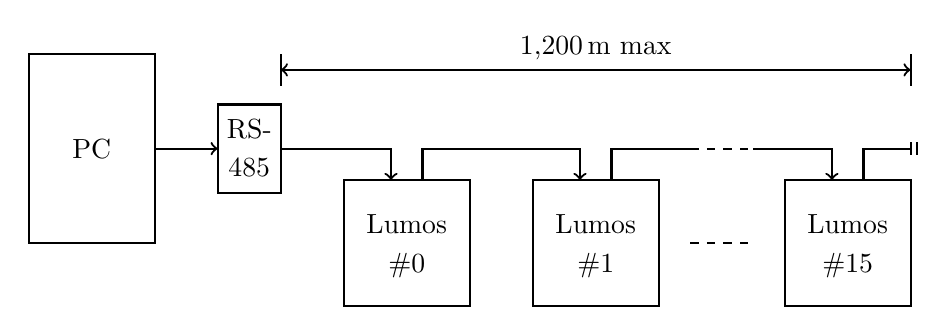
\begin{tikzpicture}[scale=.8]
		\draw [thick] (0,1) -- (0,4) -- (2,4) -- (2,1) -- cycle;
		\node at (1,2.5) {PC};
		\draw [thick] (3,1.8) -- (4,1.8) -- (4,3.2) -- (3,3.2) -- cycle;
		\node [above] at (3.5,2.5) {RS-};
		\node [below] at (3.5,2.5) {485};
		\foreach \x in {5, 8, 12} {
			\draw [thick] (\x, 0) -- (\x, 2) -- (\x+2, 2) -- (\x+2, 0) -- cycle;
			\node [above] at (\x+1, 1) {Lumos};
		};
		\node [below] at (6,1) {\#0};
		\node [below] at (9,1) {\#1};
		\node [below] at (13,1) {\#15};
		\draw [->, thick] (2,2.5) -- (3,2.5);
		\draw [->, thick] (4,2.5) -- (5.75,2.5) -- (5.75, 2);
		\draw [->, thick] (6.25,2) -- (6.25,2.5) -- (8.75,2.5) -- (8.75,2);
		\draw [thick]     (9.25,2) -- (9.25,2.5) -- (10.5,2.5);
		\draw [dashed, thick] (10.5, 2.5) -- (11.5,2.5);
		\draw [dashed, thick] (10.5, 1) -- (11.5, 1);
		\draw [->, thick] (11.5,2.5) -- (12.75, 2.5) -- (12.75, 2);
		\draw [thick]     (13.25, 2) -- (13.25, 2.5) -- (14, 2.5);
		\draw	[thick]   (14, 2.6) -- (14, 2.4);
		\draw	 [thick]  (14.1, 2.6) -- (14.1, 2.4);
		\draw   [thick]   (4, 4) -- (4, 3.5);
		\draw	[thick]   (14, 4) -- (14, 3.5);
		\draw [<->, thick] (4,3.75) -- (14, 3.75);
		\node [above] at (9, 3.75) {1,200\,m max};
	\end{tikzpicture}
	\caption{Network Connection Diagram\label{fig:net}}
\end{figure}

To connect the controllers to your PC, follow these steps:
\begin{enumerate}
	\item	Connect the \ix{RS-485 converter} to your PC's serial port using the serial cable
		which came with the converter unit.
	\item	Connect one end of an Ethernet-style cable to the \ix{RS-485} converter.
	\item	Plug the free end of that cable into the connector labeled ``\mc{IN}'' (J12) on the first Lumos
		board.  {\bfseries Note:} If you're using a weather-tight enclosure, you will need to route the cable through
		the foam grommets at the bottom of the enclosure.
	\item\label{s:net1}
		If there is more than one Lumos controller in the chain, connect one end of another 
		cable
		from the first Lumos controller's ``\mc{OUT/THRU}'' (J13) connector.
	\item\label{s:net2}
		Plug the other end of this cable into the next Lumos controller's ``\mc{IN}'' (J12) connector.
	\item	Repeat steps \ref{s:net1}--\ref{s:net2} until up to 16 Lumos controllers have been connected together.
	\item	Insert a special ``\ix{terminator plug}'' into the last Lumos controller's ``\mc{OUT/THRU}'' (J13) connector.
	\item	Refer to Figure~\ref{fig:netcables} to see how the serial network cables look
		when connected.  The unit on the left has two cables attached.  The blue cable is the incoming data line
		from the PC's RS-485 converter.  The orange cable is going out from this Lumos controller to the next one in the
		chain, which is shown on the right of Figure~\ref{fig:netcables}.  Note that on the second unit, the orange cable
		from the first unit is plugged in to the ``\mc{IN}'' jack, and a terminator plug is placed in the ``\mc{OUT}'' jack,
		ending the chain at that point.
\end{enumerate}

\begin{figure}
	\centerline{\LLimg[height=2in]{IMG387} \LLimg[height=2in]{IMG378}}
	\caption{Connected Network Cables (terminated unit on right)\label{fig:netcables}}
\end{figure}

\section{Special Instructions for RS-232 Serial Boards}\label{sec:rs232}
If your Lumos controller is built for RS-232 communications, this means it can plug directly into
your PC's standard serial port using a 9-pin serial cable.  The limitations of this kind of serial port
mean that the cable must be shielded, and not longer than 25\,ft.  Only one Lumos board may be attached
to a PC's serial port (you will need more serial ports or \mc{USB} serial adaptors to attach more Lumos
boards).

The serial cable is a standard straight-through 9-pin male-to-female configuration such as would be used
to connect a modem to your PC.

\section{Attaching Power Loads to the Lumos Controller}
Each block of 8 output channels is electrically isolated from the others, allowing them to have
separate power supplies to distribute load appropriately, or to control different voltage devices.
You must supply power to the Lumos controller itself (at connector J10) as well as to each block of 
output channels you will be controlling.

Also note that the Lumos output circuits were designed to control simple resistive loads such as
incandescent lights.  They are not appropriate for all kinds of loads.  Some inductive loads
(for example, electromagnetic relays and motors) may require a protective ``snubber'' circuit
between the Lumos output and the load to avoid damage to the Lumos board and/or the attached load.

For these instructions, we will guide you through attaching an \mc{ATX}-style \ix{power supply} to a 
Lumos board, to supply +5\,V power to run the Lumos board itself, and +12\,V to run two strings of \mc{LED}
Christmas lights.  Figure~\ref{fig:ledconn} shows how the wires are connected, using typical wire colors
employed by this style of power supply.

\begin{figure}
	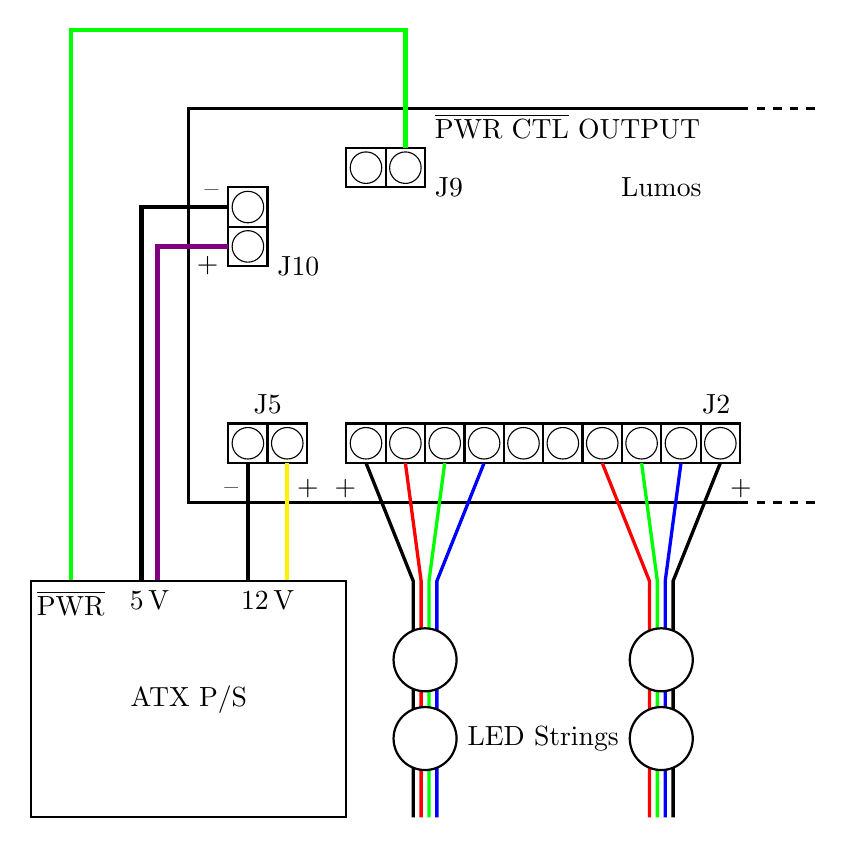
\begin{tikzpicture}
		\draw [very thick] (9,4) -- (2,4) -- (2,9) -- (9,9);
		\draw [very thick, dashed] (9,9) -- (10,9);
		\draw [very thick, dashed] (9,4) -- (10,4);
		\foreach \x in {4, 4.5} {
			\draw [thick] (\x,8) -- (\x,8.5) -- (\x+.5,8.5) -- (\x+.5,8) -- cycle;
			\draw (\x+.25,8.25) circle (.2);
		};
		\foreach \x in {2.5, 3} {
			\draw [thick] (\x,4.5) -- (\x,5) -- (\x+.5,5) -- (\x+.5,4.5) -- cycle;
			\draw (\x+.25,4.75) circle (.2);
		};
		\foreach \x in {4, 4.5, ..., 8.5} {
			\draw [thick] (\x,4.5) -- (\x,5) -- (\x+.5,5) -- (\x+.5,4.5) -- cycle;
			\draw (\x+.25,4.75) circle (.2);
		};
		\foreach \y in {8, 7.5} {
			\draw [thick] (2.5,\y) -- (2.5,\y-.5) -- (3,\y-.5) -- (3,\y) -- cycle;
			\draw (2.75,\y-.25) circle (.2);
		};
		\node [right] at (5,8) {J9};
		\node [right] at (3,7) {J10};
		\node at (8,8) {Lumos};
		\node [below left] at (2.75,4.5) {--\strut};
		\node [below left] at (4.25,4.5) {+\strut};
		\node [below right] at (8.75,4.5) {+\strut};
		\node [below right] at (3.25,4.5) {+\strut};
		\node [below left] at (2.5,7.25) {+};
		\node [above left] at (2.5,7.75) {--};
		\node [above] at (3,5) {J5};
		\node [above left] at (9,5) {J2};
		\node [above right] at (5,8.5) {$\overline{\hbox{\mc{PWR CTL}}}$ \mc{OUTPUT}};
		\draw [ultra thick, green] (0.5,3) -- (0.5,10) -- (4.75,10) -- (4.75,8.5);
		\draw [ultra thick, black] (1.4,3) -- (1.4,7.75) -- (2.5,7.75);
		\draw [ultra thick, violet]   (1.6,3) -- (1.6,7.25) -- (2.5,7.25);
		\draw [ultra thick, black] (2.75,3) -- (2.75,4.5);
		\draw [ultra thick, yellow] (3.25,3) -- (3.25,4.5);
		\draw [thick] (0,0) -- (4,0) -- (4,3) -- (0,3) -- cycle;
		\node at (2,1.5) {ATX P/S};
		\node [below] at (.5,3) {$\overline{\hbox{\mc{PWR}}}$};
		\node [below] at (1.5,3) {\mc{5\,V}};
		\node [below] at (3,3) {\mc{12\,V}};

		\draw [very thick, black] (4.85, 0) -- (4.85, 3) -- (4.25, 4.5);
		\draw [very thick, red]   (4.95, 0) -- (4.95, 3) -- (4.75, 4.5);
		\draw [very thick, green] (5.05, 0) -- (5.05, 3) -- (5.25, 4.5);
		\draw [very thick, blue]  (5.15, 0) -- (5.15, 3) -- (5.75, 4.5);

		\draw [very thick, red]   (7.85, 0) -- (7.85, 3) -- (7.25, 4.5);
		\draw [very thick, green] (7.95, 0) -- (7.95, 3) -- (7.75, 4.5);
		\draw [very thick, blue]  (8.05, 0) -- (8.05, 3) -- (8.25, 4.5);
		\draw [very thick, black] (8.15, 0) -- (8.15, 3) -- (8.75, 4.5);
		\foreach \x in {5, 8} {
			\foreach \y in {2, 1} {
				\draw [fill, white] (\x, \y) circle (.4);
				\draw [thick, black] (\x, \y) circle (.4);
			}
		};
		\node at (6.5,1) {LED Strings};
	\end{tikzpicture}
	\caption{Example Wiring of Two 12\,V R\mc{GB} L\mc{ED} Strings\label{fig:ledconn}}
\end{figure}

{\bfseries Caution:}
The colors used here are typical for \acronym{ATX} power supplies, however
not all supplies use the same color codes to mark wires.  Connecting the wrong wires to the terminals
of the Lumos board may have catastrophic consequences, including serious injury, death, fire, and severe damage
\marginpar{\centerline{\LLimg[height=.5in]{danger-generic}}}
to the controller and all devices connected to it.  Check your power supply until you are \emph{certain} you know
exactly which wires carry which signals and voltages.  Be sure your power supply has the capacity to provide the
power needed for the loads you will plug into it.

Make the main power connections to the board by following these steps:

\begin{enumerate}
	\item	Many \mc{ATX}-style power supplies have a wire which is used by the computer's motherboard
		to tell it when to start up or go to sleep (this is done to save power).  The Lumos
		board supports this feature.  If this power supply has such a wire, 
		connect it to the ``$\overline{\hbox{\mc{PWR CTL}}}$ \mc{OUTPUT}'' terminal
		\marginpar{\centerline{\LLimg[width=1.5in]{pwr-ctl-connect}}}
		J9.  Typically, this is the {\bfseries green wire} from the power supply.  

\newpage
	\item	We need to make sure the Lumos board is powered even if the power supply is in %``shutdown'' (also known as
		``sleep'' %) 
		mode.  The power supply provides a special +5\,V supply called the 
		``\ix{standby power}'' line,
		on a {\bfseries violet wire}.  Connect the violet wire to the ``+'' terminal of J10.

	\item	Connect a ground wire (typically {\bfseries black}) to the ``--'' terminal of J10.
		\marginpar{\centerline{\LLimg[width=1.5in]{logic-pwr-connect-crop}}}

	\item\label{s:pwrjump}
		Configure the input voltage jumper J17.  If the board will be provided with a regulated
		+5\,V DC supply, place a single jumper across the middle pins (2--3).  Otherwise, for input 
		supply voltages from +8\,V to +24\,V DC, place two jumpers on pins 1--2 and 3--4,
		as shown in Figure~\ref{fig:jumpers}.  In the example being described here, we are
		\marginpar{\centerline{\LLimg[width=1.5in]{IMG421}}}
		getting +5\,V so place a jumper across pins 2--3.
		\begin{description}
			\item[\HandRight\ Advanced Tip:] 
				When the voltage select jumper J17 (and the three voltage select
				jumpers J6--J8 for the output channel blocks) are in the middle position
				(pins 2--3 shorted), the on-board voltage regulator is bypassed so the
				input power is sent directly into the circuit which is expecting +5\,V.
				This is necessary because the on-board +5\,V regulator needs at least
				+8\,V input to function.  If you select this, you must supply a clean,
				regulated +5\,V source.

				When the voltage select jumpers are in the other position (pins 1--2 are
				shorted together, and 3--4 are shorted together), the input power is routed
				through the on-board regulator.  The input voltage in this case must be
				between +8 and +24\,V~DC, but need not be perfectly regulated.
		\end{description}
\end{enumerate}

Attach loads to the Lumos board by connecting them to the output channel blocks.  There are three separate
blocks of 8 channels.  Each block is independently powered via its input power terminal block (J3--J5).
When attaching power to these terminals, watch for the polarity as marked on the board.  The negative supply
is attached to the left terminal, while the positive terminal is on the right.

The eight outputs in each block are negative (--), and available at terminal blocks J0--J2.  
For your convenience, two positive (+) supply terminals
are provided on the outer two positions of each of those terminal blocks.

Follow these steps to attach the two +12\,V light strings for our example installation:

\begin{enumerate}
	\item 	Connect +12\,V to the block by attaching a {\bfseries yellow} wire from the power supply to
		the ``+'' (right) terminal of J5 on the Lumos board.

	\item	Attach another {\bfseries black} ground wire to the ``--'' (left) terminal of J5.
		\marginpar{\centerline{\LLimg[width=1.5in]{block-12v-power}}}

	\item	Configure the block's input voltage by putting jumpers on J8 as described in 
		step~\ref{s:pwrjump} on page~\pageref{s:pwrjump}.  In this example, we're using +12\,V so we place
		two jumpers onto pins 1--2 and 3--4 of J8.
		\marginpar{\centerline{\LLimg[width=1.5in]{IMG423}}}

	\item\label{s:led1}
		Attach one string of \mc{LED} lights by attaching its {\bfseries white} common wire to the ``+''
		terminal of J2.

	\item	Attach the light string's {\bfseries red} wire to the ``23'' terminal of J2.

	\item\label{s:led2}
		Repeat the previous step to attach the remaining color wires to terminals ``22'' and ``21'' on J2.

	\item	Repeat steps \ref{s:led1}--\ref{s:led2} again to attach the second string of lights to three
		more output channels (such as ``18,'' ``17,'' and ``16'') and one of the ``+'' terminals on J2.

	\item	Close the enclosure and secure it.

	\item	Plug the power supply into an AC outlet.
\end{enumerate}

\begin{figure}
    \begin{center}
	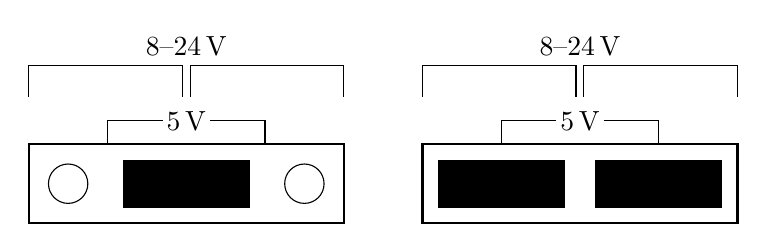
\begin{tikzpicture}
		\draw [thick] (0,0) -- (4,0) -- (4,1) -- (0,1) -- cycle;
		\draw (0.5,0.5) circle (.25);
		\draw (1.5,0.5) circle (.25);
		\draw (2.5,0.5) circle (.25);
		\draw (3.5,0.5) circle (.25);
		\draw (1,1) -- (1,1.3) -- (1.7,1.3);
		\draw (2.3,1.3) -- (3,1.3) -- (3,1);
		\node at (2,1.3) {5\,V};
		\draw (0,1.6) -- (0,2) -- (1.95,2) -- (1.95,1.6);
		\draw (2.05,1.6) -- (2.05,2) -- (4,2) -- (4,1.6);
		\node [above] at (2,2) {8--24\,V};
		\draw [fill] (1.2,0.2) -- (2.8,0.2) -- (2.8,0.8) -- (1.2,0.8) -- cycle;

		\draw [thick] (5,0) -- (9,0) -- (9,1) -- (5,1) -- cycle;
		\draw (6,1) -- (6,1.3) -- (6.7,1.3);
		\draw (7.3,1.3) -- (8,1.3) -- (8,1);
		\node at (7,1.3) {5\,V};
		\draw (5,1.6) -- (5,2) -- (6.95,2) -- (6.95,1.6);
		\draw (7.05,1.6) -- (7.05,2) -- (9,2) -- (9,1.6);
		\node [above] at (7,2) {8--24\,V};
		\draw [fill] (5.2,0.2) -- (6.8,0.2) -- (6.8,0.8) -- (5.2,0.8) -- cycle;
		\draw [fill] (7.2,0.2) -- (8.8,0.2) -- (8.8,0.8) -- (7.2,0.8) -- cycle;
	\end{tikzpicture}
	\caption{Input Voltage Select Jumpers for +5\,V (left) and +8--24\,V (right)\label{fig:jumpers}}
    \end{center}
\end{figure}

The board is now fully plugged in, connected, and ready to be controlled by the PC's software.

%\section{Performing a Field Test}
\section{Checking Your Work}
You may test the connections you made before going all the way to the PC and running a sequencing program.
This verifies that everything is working and that the lights are plugged into the correct output channels.

\begin{enumerate}
	\item	Power on the board but leave the cover open, allowing access to the control buttons.
		{\bfseries Caution:} Exercise care when working with the live board.  Don't touch anything
		\marginpar{\centerline{\LLimg[height=.5in]{danger-sign}}}
		other than the control buttons.  (Unlike the Lumos AC relay boards, your Lumos DC board
		should not normally have lethal voltages present on it, as it most often is used for small
		\mc{LED} lights powered by a few milliamps at 5 or 12 volts; however, your specific application
		may involve plugging in more dangerous levels of current, even at low voltages.  We still 
		advise caution in all cases.)

	\item	Check that the green \mc{LED} on the Lumos controller is slowly fading on and off.  This indicates
		that the controller is in its normal operating mode and is functioning correctly.

	\item	Press and hold the green ``{\mc{OPTION}}'' button until the Lumos board's diagnostic lights all start
		\index{button, option}
		flashing rapidly.

	\item	Release the button and wait a second or two for the lights to change to just the green light
		flashing rapidly (the others will be off).  
		The Lumos board is now in ``\ix{configuration mode}.''

	\item	Press the green ``{\mc{OPTION}}'' button again for at least 2~seconds.
		\index{button, option}

	\item	Release the button.  The green light will turn off, and the red light will pulse rapidly.
		The Lumos board is now in ``\ix{field test mode}.''
\end{enumerate}

This mode is designed to help you check your connections before closing up the units and starting your
show.  The controller will cycle each output channel on for one second, then off again, starting with channel 0.  
Each second, the next channel in order from 0--23 will turn on, then wll restart with channel 0 again.

When you're finished with this test, simply press the red ``\mc{RESET}'' button to reset the controller
\index{button, reset}
back to normal operating mode.

\begin{description}
	\item[\HandRight\ Tip:]  You can ``freeze'' the cycle, holding the currently-lit
		output channel on indefinitely, by pressing the green ``\mc{OPTION}'' button
		briefly.  Press it again to resume the test cycle.
\end{description}

\chapter{Going On From Here}
Now that your controller is installed and ready to use, refer to the separate manual,
\emph{Using Lumos SSR Controllers} for full instructions on how to program
and use your controller with your computer or in stand-alone operation.

%\section{Getting Additional Help}
The \ix{product website} at \URL{www.alchemy.com/lumos} contains additional documentation,
\index{website}
pointers, hints, and tips to assist you further.  If that doesn't answer all your questions,
there is an \ix{online forum} where you may submit questions for help.

\backmatter
\appendix

\input pinouts

\chapter{Troubleshooting}\label{ch:troubleshooting}
%\LLstart{W}{HILE}{we anticipate} 
While we anticipate the Lumos board will provide many hours of worry-free operation,
as with any device (particularly one built as a \acronym{DIY} project), sometimes things don't go
quite as planned.  Here are a few common problems and their solutions.

\begin{longtable}{|p{1.5in}|p{1.5in}|p{2in}|}\hline
\bfseries Symptom & \bfseries Likely Cause(s) & \bfseries Solution \\\hline\hline
\endhead
An entire block of outputs does not turn on 
	& No power to the block 
	& If the \mc{BLOCK PWR} light is off, check the fuse for that block, 
	  the connection from the power supply to the block, and that the power supply is powered on.\\
\cline{2-3}
	& Power supply not told to wake up (\mc{ATX}-style supplies only).
	& Check that the power supply's green wire is attached to the $\overline{\hbox{\mc{PWR CTL}}}$
	  terminal on J9. \\\hline
Some outputs don't work, or are erratic.
	& Loose % opto-isolator 
chip.
	& Lightly press chips U0--U5 back into their sockets.\\
\cline{2-3}
	& Bad solder connection or loose chip.
	& Re-check all solder connections on the board, re-solder any which are cold, broken, or
	  incomplete.\\\hline
No units in serial network respond to commands.
	& Missing terminator
	& Replace terminators on both ends of the daisy chain (note the PC's RS485 converter
	  may include a built-in terminator for that position).\\\hline
One unit does not respond to commands.
	& Wrong address.
	& Use the \verb+lumosctl+ program to reconfigure the board to have
	  the correct address.\\
\cline{2-3}
	& Blown communication fuse.
	& Replace fuse F3.\\\hline
\end{longtable}


%\chapter{Diagnostics}\label{ch:diagnostics}


\chapter{Glossary}\label{ch:glossary}
\begin{description}
	\item[Active High:]
		A logic signal which is considered ``on'' when the signal is ``high'' (binary 1 or +5\,V),
		and ``off'' when the signal is ``low'' (binary 0 or 0\,V).  Lumos relay circuits are 
		triggered with active-low signals.
	\item[Active Low:]
		A logic signal which is considered ``on'' and ``off'' at the opposite signal levels
		to an ``active high'' signal (q.v.).
%	\item[Annular Ring:]
%		The exposed ring of metal around a hole in a \acronym{PCB} where a component is to be 
%		mounted.  The solder will flow across the component lead and onto the annular ring.
	\item[Daisy Chain:]
		The arrangement of wiring a number of devices together by connecting the first to the second,
		then adding another connection from the second to the third, and so forth.  The network
		connection diagram in Figure~\ref{fig:net} shows an example of a daisy chain.
%	\item[\acronym{DIP} (Dual In-line Package):]
%		The style of chip where the pins are laid out in two parallel rows.
	\item[\acronym{DCE} (Data Communications Equipment):]  In the realm of RS-232 devices, this is the peripheral
		device plugged into the main ``terminal'' (\acronym{DTE}) device.  Examples include
		Lumos controllers and modems.
	\item[\acronym{DIY}:] ``Do-It-Yourself.''
	\item[\acronym{DTE} (Data Terminal Equipment):]  In the realm of RS-232 devices, this is the
		main ``terminal'' device such as a PC or teletype.
	\item[Duplex:]
		a feature of a serial line.  On a full-duplex connection, separate data wires are present
		to carry data in both directions, so one device can send and receive data at the same time.
		On a half-duplex connection, only a single set of data wires is present, so devices must
		take turns transmitting over them.
	\item[\acronym{ESD} (Electro-Static Discharge):]
		static electricity which builds on your skin and is then discharged into sensitive
		components when you touch them.  Invisible to the eye, this can punch microscopic holes
		in the inside of the components, severely damaging them.
%	\item[Heat Protection:]
%		A temporary heat sink applied to a component when soldering that component onto
%		the \acronym{PCB}.  Typically used for heat-sens\-i\-tive components such as transistors
%		and integrated circuit chips.
	\item[Jumper Block:]
		A series of pins mounted to the \acronym{PCB}.  Different options are configured for the
		circuit by placing a jumper over certain pairs of pins, shorting them together.
	\item[\acronym{LED} (Light Emitting Diode):]
		A special kind of diode which emits light when current passes from its anode to its cathode.
%	\item[\acronym{MOSFET}:]
%		The type of transistor which forms the major part of a Lumos DC relay channel.  The name
%		is an acronym for Metal Oxide Semiconductor Field Effect Transistor.
	\item[\acronym{PCB} (Printed Circuit Board):]
		The board where electronic components are mounted to form a complete circuit.  Metal
		traces are ``printed'' (actually etched) onto the surface of the board itself to make the
		connections between components.
	\item[RS-232:]
		A standard hardware protocol for sending serial data between two devices (such as a computer
		and a modem or a single Lumos board).  Shielded cable should be used for best results, and
		the cable length should not exceed 25\,ft.
	\item[RS-485:]
		A standard hardware protocol for sending serial data between multiple devices on a single
		cable length (electrically it is a single cable which each device ``taps into'' along the
		line; physically it is typically a ``daisy chain'' arrangement where a short cable connects
		one device to the next, another cable to the next, and so on). Unshielded twisted-pair cable
		is used (like Ethernet cable), and the cable lengths should not exceed a total of 4,000\,ft
		(1,200\,m).
	\item[Terminator Plug:]
		An RS-485 network requires a terminator at each end.  This is a small plug which plugs into
		the last unit in the daisy chain.
	\item[\acronym{TTL} (Transistor-Transistor Logic):] One of the ways digital logic circuits can be
		constructed.  For our purposes here, we consider a ``\acronym{TTL}-level'' signal to be a
		logic input or output where a voltage near +5\,V is ``high'' (binary 1 or ``true'') and a
		voltage near 0\,V is ``low'' (binary 0 or ``false'').  The inputs should never be above
		+5 nor below 0 volts.
\end{description}

\input acknowledgements 

\indexintoc
\printindex
\clearpage

\input colophon
\end{document}
